%\documentclass{report}	
\documentclass[10pt]{article}	
\usepackage[paperwidth=21cm, paperheight=29.7cm,top=10mm, bottom=10mm, left=17mm, right=12mm]{geometry} %dont use, overrides many options
%\usepackage[figuresright]{rotating}
\usepackage{algorithmic}
\usepackage{algorithm}
\usepackage{booktabs}
\usepackage{enumitem}
%\usepackage{html}
\usepackage{url}
%\usepackage{wrapfig}
\usepackage{color}
%\usepackage{array}
%\usepackage{textcomp}
%\usepackage{longtable}
\usepackage{amsmath}
\usepackage{amsfonts}
\usepackage{amssymb}
\usepackage{graphicx}    
%\usepackage{microtype}    % improves line-breaks in narrow columns
\usepackage{enumitem}
\usepackage{subfig}
%%\usepackage{cite}
%\usepackage{eucal}
\usepackage[export]{adjustbox}
\usepackage{dirtree}
%\usepackage[colorinlistoftodos,textwidth=0.95\marginparwidth]{todonotes} % To add in-line review comments
%\usepackage{changes}
\usepackage[font=small,skip=0pt]{caption}
\usepackage[affil-it]{authblk}
\usepackage{natbib}
\setlength{\bibsep}{0pt plus 0.3ex}
\usepackage{titlesec}
\titlespacing\section{0pt}{12pt plus 8pt minus 2pt}{0pt plus 8pt minus 2pt}
\titlespacing\subsection{0pt}{12pt plus 4pt minus 2pt}{0pt plus 2pt minus 2pt}
\titlespacing\subsubsection{0pt}{12pt plus 4pt minus 2pt}{0pt plus 2pt minus 2pt}


\title{\vspace{-12mm} Computing a well-connected Midsurface} % Your article title

\author{Yogesh Kulkarni%
  \thanks{E-mail: \texttt{kulkarniyh12.mech@coep.ac.in}, Profile: \texttt{https://www.linkedin.com/in/yogeshkulkarni}, Phone: \texttt{+91 9890251406}}}
\affil{PhD Student, Department of Mechanical Engineering, College of Engineering Pune, India.}

\date{} % Add a date here if you would like one to appear underneath the title block

\begin{document}

\maketitle

\vspace{-12mm}
\section{Introduction}\label{sec:intro}

Getting a quicker validation of the proposed product is crucial in the era of fierce competition and faster obsolescence. Digital product development, which includes, modeling by CAD (Comouter-aided Design)  and analysis by CAE (Computer-aided Engineering) plays a crucial role in quicker ``Time to market''.  For thin-walled models such as sheet-metal/plastic products, a quicker and fairly accurate CAE analysis is possible by idealizing them to their equivalent surface representations, called ``Midsurface''. Midsurface can be envisaged as a surface lying midway of a thin-walled solid, mimicking its shape.   In CAE analysis, instead of using expensive 3D solid elements, 2D surface elements are used on the midsurface for fairly accurate results in lesser computations/time.  Even in the age of scalable and near-infinite computing power, it is still desirable to have  a robust, well-connected midsurface, so as to be able to run more design iterations, quickly.  Because of such advantages, the midsurface functionality is widely used and is available in many commercial CAD-CAE packages. 

\begin{minipage}[h]{\linewidth} 
\begin{minipage}[h]{0.5\linewidth} 
		\centering
		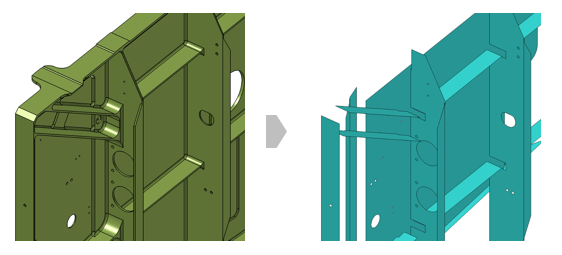
\includegraphics[width=0.9\linewidth]{../images/MidsurfaceErrorsMscApex}
		\captionof{figure}{Midsurface Errors (Source: \cite{MScApex})}
		\label{fig:midsurfaceerrors}
\end{minipage}
\hfill
\begin{minipage}[h]{0.5\linewidth} 
In spite of its demand and popularity, the existing techniques of computing the midsurface fail to compute a well-connected midsurface, especially for non-trivial shapes (\cite{Woo2013,Automex}). Failures manifest in the form of gaps, missing patches, overlapping surfaces, not lying midway, not mimicking the input shape, etc. (Figure \ref{fig:midsurfaceerrors}). Correcting these errors is mostly a manual, tedious and highly time-consuming task, requiring hours to days. This correction time can be nearly equivalent to the time it can take to create the midsurface manually from scratch (\cite{Stolt2006}). 
\end{minipage}
\end{minipage}
%\end{figure}



 Automated and  robust technique for computing midsurface  is a crucial need and this work is a step in that direction. Simplification, abstraction and decomposition are the core themes of the proposed approach.


\section{Proposed Approach}
\label{sec:approach}
The input  (Figure \ref{fig_sysarch}) is a feature-based CAD model represented by  ($\cup_qf^3$), where `$\cup$' denotes a collection, of `$q$' features (`$f$') having dimensionality `$3$' (solids). In practice, the thin-walled CAD models come in various types, such as mesh, solid, feature-based CAD, etc. This research, as it leverages feature information \cite{YogeshCOEP2013}, expects a feature-based CAD model as input. This, at times can be deemed as limitation, in case of unavailability due to format restrictions, proprietary data etc. But, techniques such as segmentation, feature recognition (FR), can be used effectively to convert the non-feature-based model to a feature-based one.

%\smallskip

\begin{minipage}[c]{\linewidth}
    \begin{minipage}[c]{0.45\linewidth}
\begin{itemize}[noitemsep,topsep=2pt,parsep=2pt,partopsep=2pt,leftmargin=*]
%\item \textbf{Input}: Feature-based CAD models, which are widely available in most of the commercial CAD applications. It is represented by  ($\cup_qf^3$), where `$\cup$' denotes a collection, of `$q$' features (`$f$') having dimensionality `$3$' (solids). Thin-walled CAD models come in various representations, such as mesh, solid, feature-based, etc. This research expects a feature-based CAD model, which can be deemed as limitation in case of its unavailability. But, techniques, such as segmentation, decomposition, feature recognition (FR), etc. can convert a non-feature-based representation to the feature-based CAD model.

\item \textbf{Defeaturing ($\cup_rf^3, r \leq q$) }:  Computes gross shape by removing irrelevant/superficial features \cite{YogeshIITM2013}, using Feature taxonomy and size-based Remnant feature approach (\cite{YogeshCADConf2015}). 

\item \textbf{Generalization ($\cup_rL^3$) }: ``ABEL'' transforms form-features to ``Loft/Sweep'' representations ($L$), making it simpler to develop a generic, portable algorithm (\cite{YogeshIITG2014}). 

\item \textbf{Decomposition}: Cellular decomposition is performed at each feature step to form a graph of nodes having non-volumetrically-overlapping cellular bodies with respective owner-Sweep feature. 

\item \textbf{Midsurface Computation}: Using topology of the graph, the nodes are classified into midsurface-patch generating nodes (solid cells - $sCell$s) and interaction-resolving nodes (interface cells - $iCell$s). Midsurface patch is computed by, first, extracting the profile and the guide curve from the owner Sweep feature, then either offsetting the profile in case of shorter guide curve or sweeping the midcurve \cite{YogeshETES2014,YogeshIJCAET2017} along the guide curve.

\item \textbf{Validation}:  Midsurface needs to  mimic the input shape, faithfully. A novel topological method is used to validate correctness of the midsurface (\cite{YogeshCADandA2015}).

%\item \textbf{Output}: A well-connected midsurface is then sent to downstream applications such as CAE analysis.
\end{itemize}



    \end{minipage}
    \hfill
    \begin{minipage}[c]{0.5\linewidth}
	\centering 
	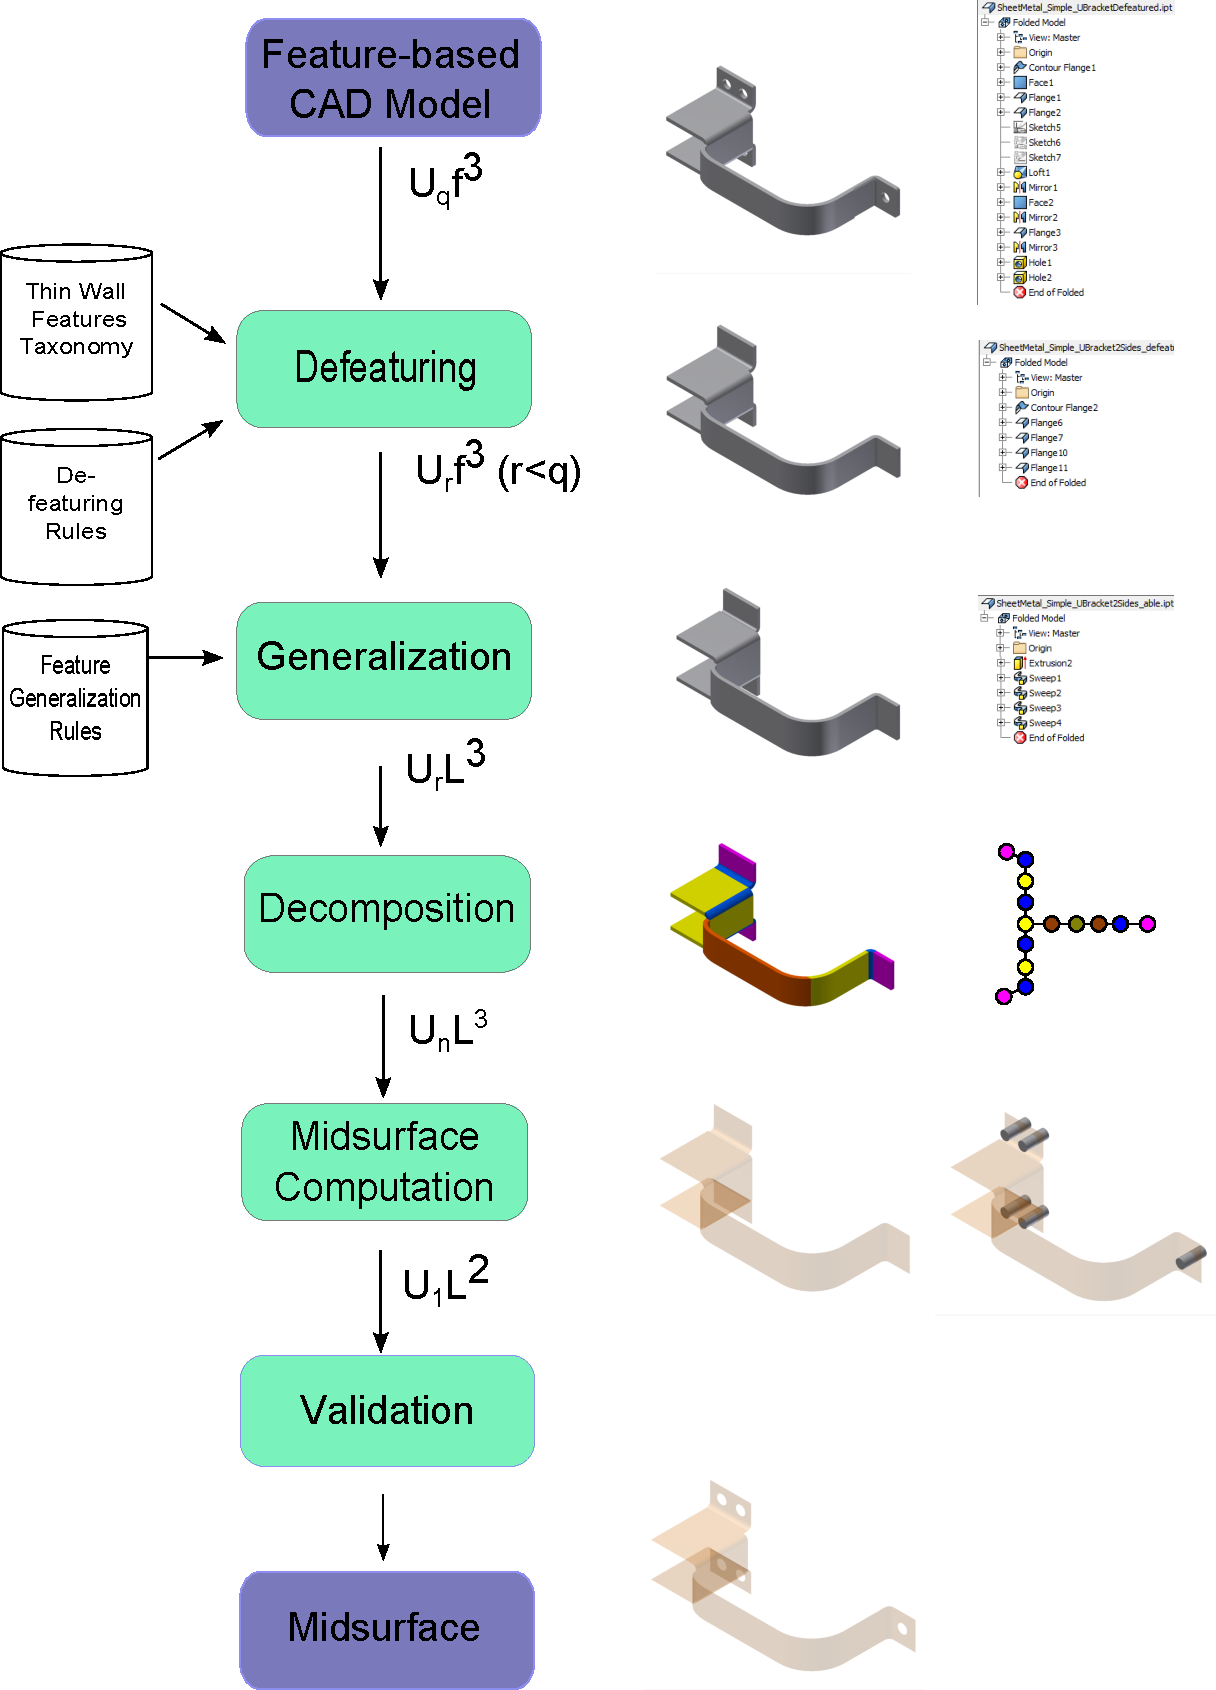
\includegraphics[width=0.95\linewidth]{../images/SystemArchitecture3.pdf}
	\captionof{figure}{Overall work-flow}
	\label{fig_sysarch}
    \end{minipage}

\end{minipage}    

A well-connected output midsurface is then sent to downstream applications such as CAE analysis. 

%\bigskip



\section{Conclusion}

Computation of midsurface is one of the popular simplification techniques for CAE analysis of  thin-walled models. In-spite of good demand, current methods (especially the popular Midsurface Abstraction - MA) suffer from problems such as gaps, overlaps, not lying midway, improper connections, etc.  In MA, these failures are due to complexities of face-pair detection and interactions. In our approach uses feature simplification and abstraction to resolve face-pair detection problems and  cellular decomposition to develop a generic logic to address interaction problems amongst midsurface patches. 

%\vspace{-5mm}

\begin{figure}[htp]
\centering     %%% not \center
\subfloat[Original Part]{\label{fig_orig}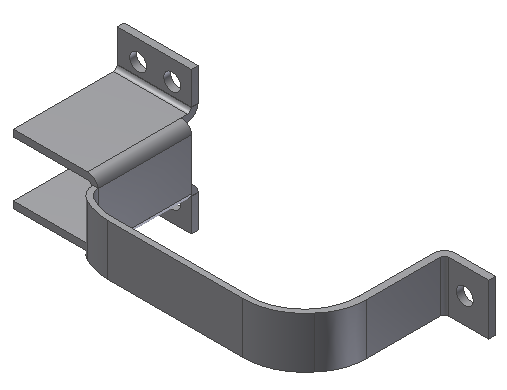
\includegraphics[width=0.23\linewidth,valign=t]{../images/nonCellularBracket}} \quad
\subfloat[Decomposition]{\label{fig_cd}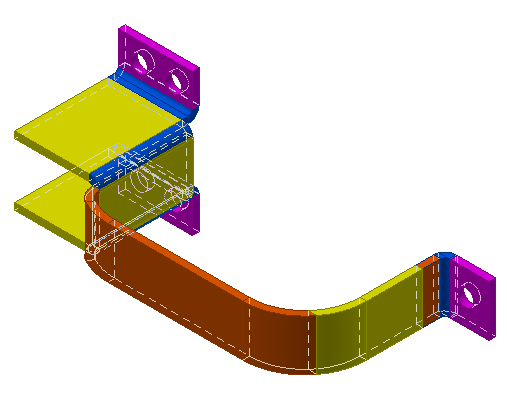
\includegraphics[width=0.23\linewidth,valign=t]{../images/CellularBracket}}\quad
\subfloat[Graph]{\label{fig_cg}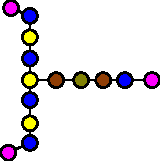
\includegraphics[width=0.175\linewidth,valign=t]{../images/CellGraphBracket.pdf}} \quad
\subfloat[Midsurface]{\label{fig_mids}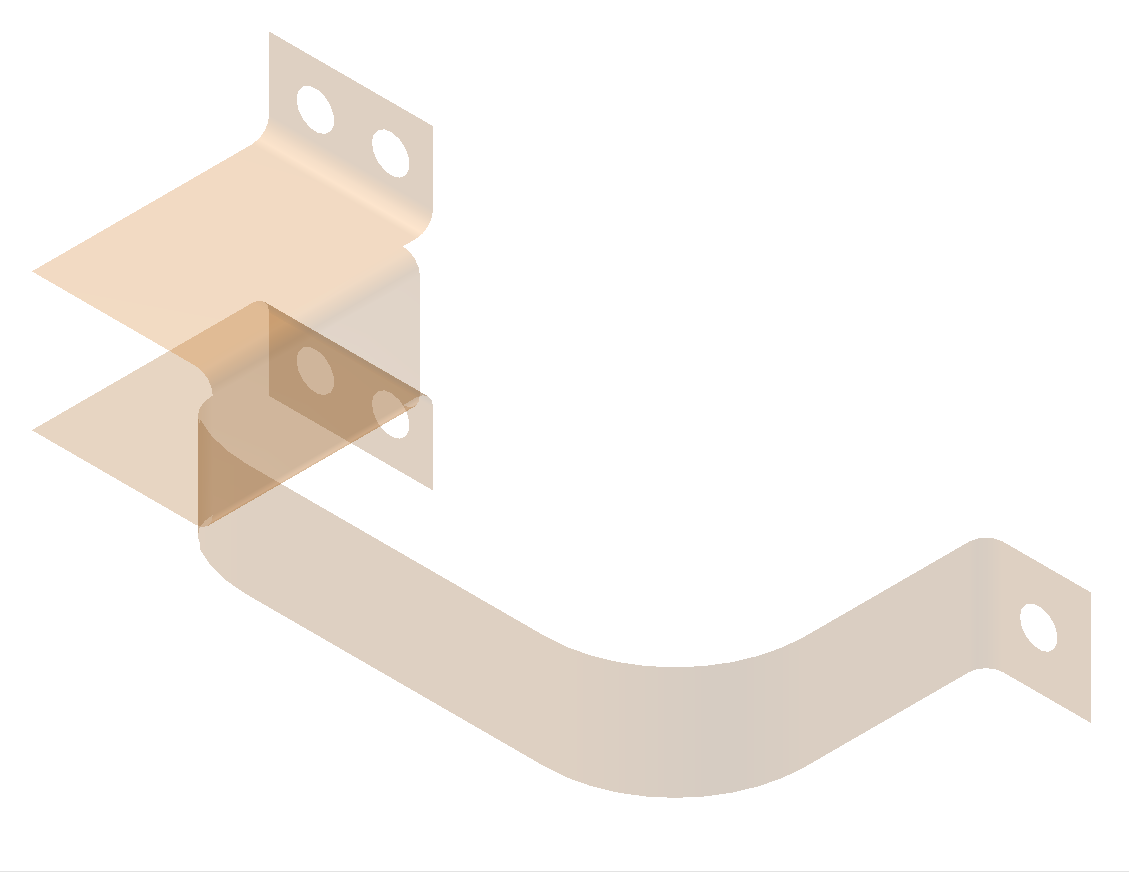
\includegraphics[width=0.23\linewidth,valign=t]{../images/MidsurfAfterDormant}}
\end{figure}


Following is a  comparative analysis of some relevant approaches vis-a-vis our approach:

\begin{table}[htp]
%\tiny
  \centering 
\resizebox{0.8\linewidth}{!}{ 
\begin{tabular}[htp]{@{} p{0.1\linewidth} p{0.2\linewidth}  p{0.2\linewidth} p{0.2\linewidth} p{0.2\linewidth}@{}}
\toprule
\textbf{Researcher}  &	\textbf{Method} &	 \textbf{Shortcomings}  &	 \textbf{Our Approach}\\ \midrule
\textbf{Chong et al.} \cite{Chong2004}  & 
Uses concave edge decomposition. Midcurves by collapsing edge pairs. If they form a loop, creates a midsurface patch & 
Hard-coded inequalities/values to detect edge-pairs. Connection logic is not generic and comprehensive &
A generic treatment for the computation of midcurves, midsurface patches and their connections
\\ \midrule
 \textbf{Boussuge et al.} \cite{Boussuge2014}  & 
 Generative decomposition. Recognizes Extrudes of each sub-volume. Creates midsurface patches in each and connects them together. &
 
 \begin{itemize}[noitemsep,nosep,leftmargin=*]
\item No fillets/chamfers.
\item Only Additive cells.
\item Only Extrudes with Analytical surfaces
\item Expensive MAT to detect thin profiles
\item Works only on Parallel and Orthogonal connections.
\end{itemize}
&
\begin{itemize}[noitemsep,nosep,leftmargin=*]
\item No such restriction
\item Re-inserts -ve cells
\item Generic Sweep extend-able to Loft
\item Simple rules of size of profile/guide
\item Generic logic for any numbers/types of connections.
\end{itemize}

\\ \midrule

\end{tabular}
}
% \caption{Comparison with Other Simplification Methods}
%  \label{tab:defeat_test}
\end{table}


%\vspace{-8mm}

\bibliographystyle{abbrv}
\bibliography{bibliography}

\end{document}